\documentclass[letterpaper,10pt]{article}

\usepackage[utf8]{inputenc}
\usepackage[spanish]{babel}
\usepackage{fontenc}
\usepackage[dvipdfmx]{graphicx}
\usepackage{bmpsize,wrapfig,xcolor}
\usepackage{fullpage}
\usepackage{amssymb}
\usepackage[hidelinks]{hyperref}

% Para evitar que se indente solo a cada rato
\setlength\parindent{0pt}

\begin{document}
	\begin{titlepage}

		\begin{wrapfigure}{R}{0.3\textwidth}
			
\includegraphics[width=0.3\textwidth]{logoFCFM.png}
		\end{wrapfigure}

		\noindent \phantom - % "Hax" para que quede alineada la imagen con el texto

		Universidad de Chile

		Facultad de Ciencias Físicas y Matemáticas

		Depto. de Ciencias de la Computación

		CC4102 - Diseño y Análisis de Algoritmos

		\vfill

		\begin{center}
			\begin{Huge}
				{\textbf{Tarea 3}}
			\end{Huge}
		\end{center}

		\vfill

		\begin{flushright}
			\begin{tabular}{lll}
				Integrantes	&:	& Americo Ferrada\\
						&	& Belisario Panay\\
				Profesor	&:	& Pablo Barcelo\\
				Ayudantes	&:	& Claudio Torres\\
						&	& Jaime Salas\\
				Auxiliar	&:	& Ariel Cáceres\\
			\end{tabular}
		\end{flushright}

	\end{titlepage}

	% % % % % % % % % % % % % % % % % % % % % % % % % % % % % % % % % % % % % % % % % % % % % % % % % % % % % % % % % % % % % % % % % % % % % % % % % % % % % % % % % % % % % % % % % %
	\newpage
	% % % % % % % % % % % % % % % % % % % % % % % % % % % % % % % % % % % % % % % % % % % % % % % % % % % % % % % % % % % % % % % % % % % % % % % % % % % % % % % % % % % % % % % % % %

	\tableofcontents

	% % % % % % % % % % % % % % % % % % % % % % % % % % % % % % % % % % % % % % % % % % % % % % % % % % % % % % % % % % % % % % % % % % % % % % % % % % % % % % % % % % % % % % % % % %
	\newpage
	% % % % % % % % % % % % % % % % % % % % % % % % % % % % % % % % % % % % % % % % % % % % % % % % % % % % % % % % % % % % % % % % % % % % % % % % % % % % % % % % % % % % % % % % % %

	\section{Introducción}

	En el presente informe se muestra el diseño, implementación y exvaluación y comparación en la práctica de tres enfoques para encontrar una solución aproximada dle problema de Cubrimiento de Vértices Mínimo, el primero la 2-aproximación vista en clases, el segundo la heurística vista en clase auxiliar y por ultimo un tercer enfoque que utiliza ambos enfoques.\\

	 Para esta tarea se comprarán el tamaño de los resultados entregados por las tres aproximaciones antes explicados. Para esto se correran los experimentos en grafos de distintos tamaños, creando grafos de manera aleatoria con una probabilidad de que dos vertices esten conectados, para así obtener promedios confiables. 
	
	\subsection{Problema a resolver}

	Encontrar el Cubrimiento por Vértices Mínimo es un problema np-Completo por lo que no puede ser usado en la práctica, para esto se ocupan los algoritmos aproximados que entregan una solucion a este problema con ciertas garantias (distancia máxima del optimo). 

	\subsection{Hipótesis}
	
	
	En general se espera que la cantidad de vertices encontrados por los tres algoritmos, aumente en función del valor de \textit{p}, esto es, mientras exista una probabilidad mayor de que una arista pertenezca al grafo, mayor será el tamaño de las soluciones.
	\\\\
    La 2-aproximación tomará menor tiempo de ejecución que las otras dos aproximaciones, pero entregará mayor cantidad de vertices que la solución de la 2-Aproximacion mejorada.
    \\\\
    Para el caso de la Heurística, se espera que la cantidad de vertices entregados sean dependientes de la entrada. 
    \\\\
    Por último para la 2-Aproximación mejorada, se cree que ocupando parte de los dos enfoques anteriores, entregará mejores resultados que las otras aproximaciones, aunque se espera que no se diferencie mucho de la 2-Aproximación.
	
	

	

	% % % % % % % % % % % % % % % % % % % % % % % % % % % % % % % % % % % % % % % % % % % % % % % % % % % % % % % % % % % % % % % % % % % % % % % % % % % % % % % % % % % % % % % % % %
	\newpage
	% % % % % % % % % % % % % % % % % % % % % % % % % % % % % % % % % % % % % % % % % % % % % % % % % % % % % % % % % % % % % % % % % % % % % % % % % % % % % % % % % % % % % % % % % %

	\section{Diseño Teórico}
    
    En esta sección se mostrará la estructura utilizada para representar el grafo, además de la descripción de las clases utilizadas en la implementación.
	
	Para representar el grafo, se dicidió utilizar la estructura presentada por el profesor \href{https://users.dcc.uchile.cl/~jfuentess/}{José Fuentes}, el cual representa el grafo con dos arreglos, un arreglo de aristas $E_G$ (una lista de adyacencia), las cuales poseen una arista y otra complementaria (ej: (u,v) y (v,u)), cada arista posee un \textit{source} o src (vertice del que proviene) y un \textit{target} o tgt (vertice al que va), además de que cada una posee el indice de su arista complementaria (cmp). Tambien posee un arreglo de vertices $V_G$, donde cada vertice posee el inicio y final de donde se encuentra en la lista de aristas. Para una mayor comprensión se muestra la siguiente figura.\\
	
	
		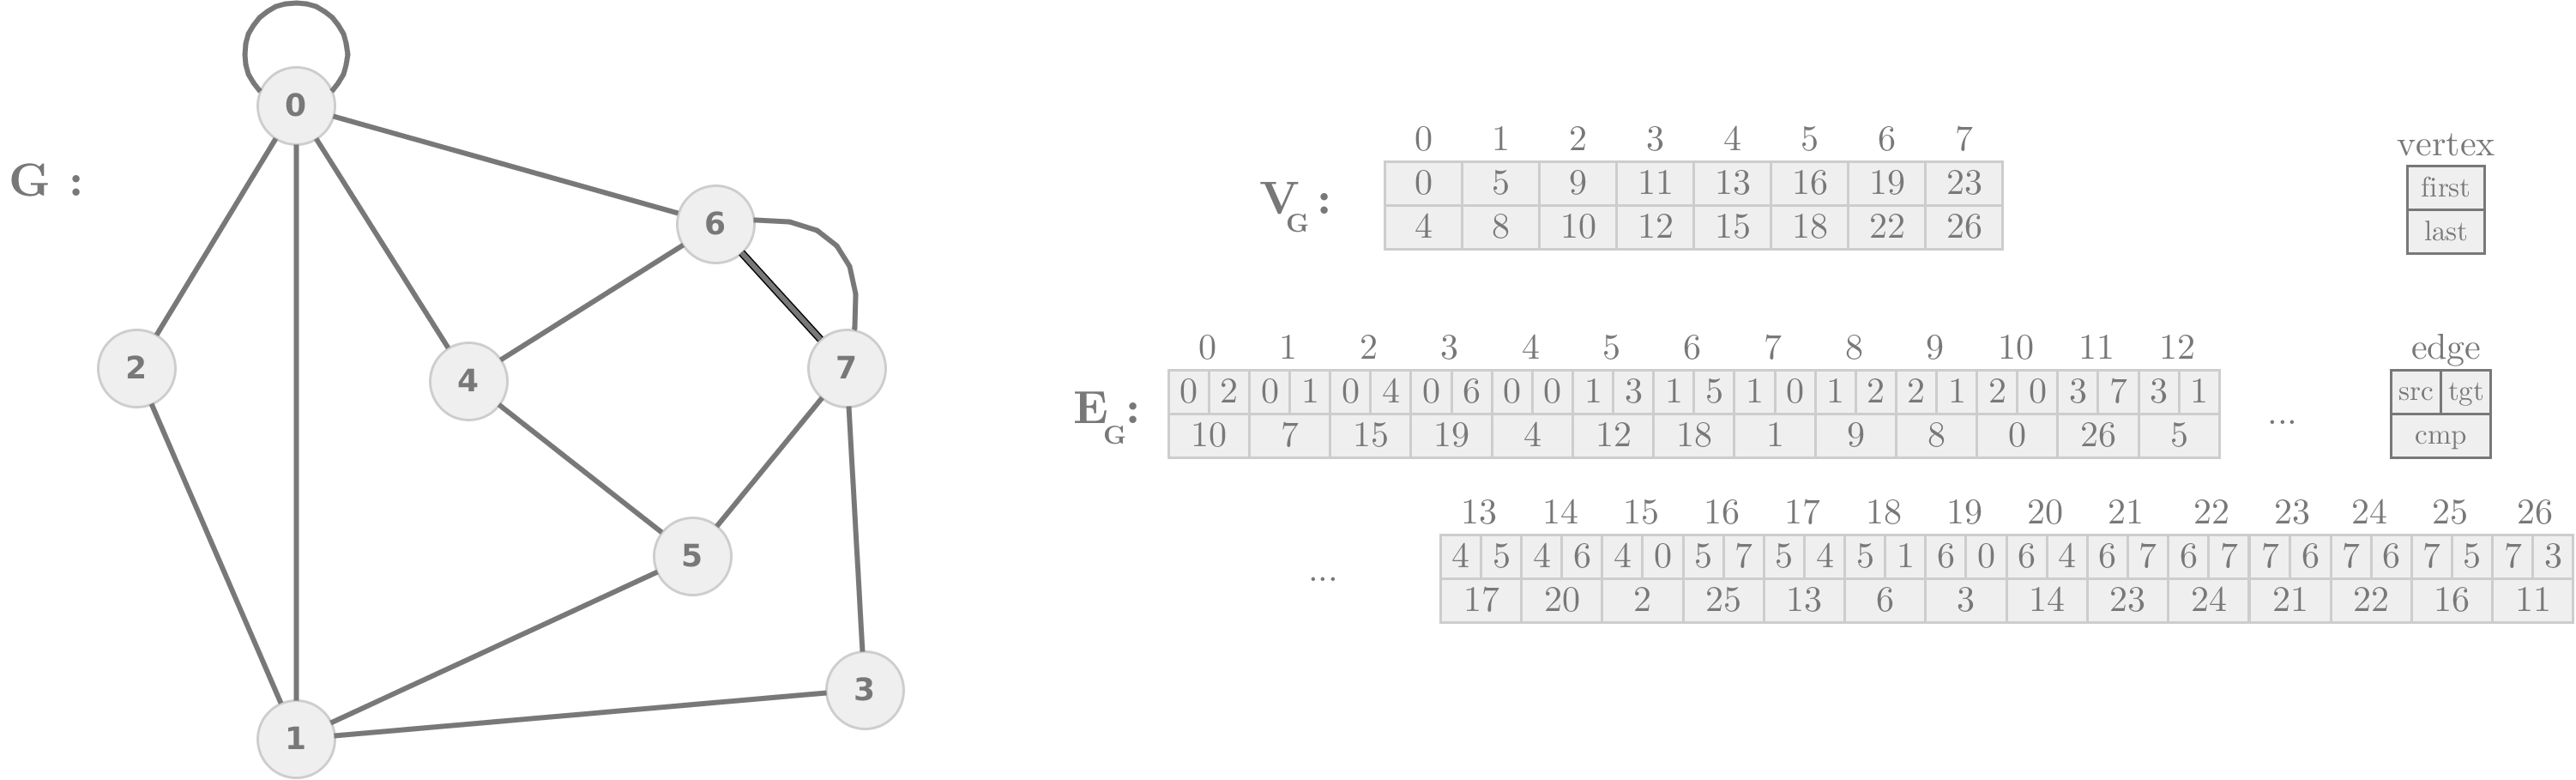
\includegraphics[width=0.8\textwidth]{figura1.png}
	\\
	
	Para los experimentos se pidió utiliar cinco distintas probabilidades para la probabilidad de que exista una arista, se utilizaron los siguientes valores 
	

  \begin{center}
		\begin{tabular}{|c|}
			\hline
			$p$\\
			\hline
			$0.00005$ \\
			\hline
			$0.0001$\\
			\hline
			$0.0005$\\
			\hline
			$0.001$\\
			\hline
			$0.05$\\
			\hline
			
		\end{tabular}
	\end{center}
	
	
	Que para todo $n = 2^i$ con $i\in{10,11,...,20}$, p se encuentra en el intervalo $[1/n,1]$ como se pidió.

	
	
	\subsection{Main}
	
	En Main se obtendran los archivos donde se registrán los tiempos de creación de los grafo, la ejecucion de los tres algoritmos, además de la cantidad de vertices que cada algoritmo obtiene para poder cubrir el grafo, para luego poder graficar. Para esto se hizo lo siguiente.
	\begin{itemize}
		\item Primero se definen las variables a utilizar al iterar.
		\item Se itera sobre los valores de $i$, creando dos archivos, un archivo de texto para poder ser leido por una persona y otro en formato CSV para poder ser leido por un software para luego ser graficado. 
		\item En cada iteración sobre $i$ se hacen tres experimentos por cada valor de $p$.
		\item En cada uno de estos experimentos sobre un $p$, se genera un grafo aleaotrio midiendo su tiempo de contrucción y se crean dos copias de esta para que cada algoritmo trabaje con una copia (pudiendo cambiarla).Luego se ejecuta cada algoritmo midiendo sus tiempos de ejecucion y registrando la cantidad de vertices de su solución.
		
	\end{itemize}

	\subsection{Graph}

	Preprocesa el texto para eliminar todos los caracteres que no serán utilizados en los experimentos, además elige aleatoriamente palabras pertenecientes al texto.

	Posee 3 métodos auxiliares:
	\begin{itemize}
		\item clean(): Elimina del texto todos los caracteres que no serán utilizados.
		\item getRandomWord(ArrayList<String> words): Dato una lista elige un elemento de manera aleatoria.
		\item getNextRandom(): Entrega palabras del texto, como una \textit{queue}. 
	\end{itemize}

	\subsection{Vertex}

	Crea el suffix array y también realiza la busqueda de un patrón sobre este.
	
	\begin{itemize}
		\item constructArray(int[] text, int n, int alphabet): Recive un texto representado con enteros y el tamaño del alfabeto, retorna el arreglo de sufijos (como arreglo de enteros).
		\item sort(int[] a, int[] array, int n, int buckets) : Radix Sort de una lista de triplas de caracteres en un alfabeto, usando counting sort.
		\item getNextRandom(): Entrega palabras del texto, como una \textit{queue}.
		\item findPattern(String pattern): Esta funcion encuentra las posiciones en el texto donde se puede encontrar el  patron, haciendo busqueda binaria en el suffixArray y en cada busqueda binaria comparando el patron con el sufijo, caracter a caracter.
	\end{itemize}

	\subsection{Edge}

	Esta clase crea un automata recibiendo un \textit{String} y crea la tabla de transiciones.
	
	\begin{itemize}
	 \item getCantRepeticiones(): Entrega la cantidad de repeticiones del patrón en el texto.
	\end{itemize}
	
	\subsection{GraphGenerator}

	Esta clase crea un automata recibiendo un \textit{String} y crea la tabla de transiciones.
	
	\begin{itemize}
	 \item getCantRepeticiones(): Entrega la cantidad de repeticiones del patrón en el texto.
	\end{itemize}
	
	\subsection{TwoAproximation}

	Esta clase crea un automata recibiendo un \textit{String} y crea la tabla de transiciones.
	
	\begin{itemize}
	 \item getCantRepeticiones(): Entrega la cantidad de repeticiones del patrón en el texto.
	\end{itemize}
	
	\subsection{MaximumDegreeHeuristic}

	Esta clase crea un automata recibiendo un \textit{String} y crea la tabla de transiciones.
	
	\begin{itemize}
	 \item getCantRepeticiones(): Entrega la cantidad de repeticiones del patrón en el texto.
	\end{itemize}
	
	\subsection{ImprovedTwoAproximation}

	Esta clase crea un automata recibiendo un \textit{String} y crea la tabla de transiciones.
	
	\begin{itemize}
	 \item getCantRepeticiones(): Entrega la cantidad de repeticiones del patrón en el texto.
	\end{itemize}



	% % % % % % % % % % % % % % % % % % % % % % % % % % % % % % % % % % % % % % % % % % % % % % % % % % % % % % % % % % % % % % % % % % % % % % % % % % % % % % % % % % % % % % % % % %
	\newpage
	% % % % % % % % % % % % % % % % % % % % % % % % % % % % % % % % % % % % % % % % % % % % % % % % % % % % % % % % % % % % % % % % % % % % % % % % % % % % % % % % % % % % % % % % % %

	\section{Presentación de los Resultados}

	\subsection{Tiempo de Creación y Búsqueda del Suffix Array}

	Los resultados para los tiempos de construcción del Suffix Array, fueron los siguientes.

	\begin{center}
		\begin{tabular}{|c|c|}
			\hline
			Tamaño del texto (Kb) ( & Tiempo de Construcción (ms)\\
			\hline
			$250$ & 210,398\\
			\hline
			$500$ & 384,365\\
			\hline
			$1000$ & 562,266\\
			\hline
			$2000$ & 2345,070\\
			\hline
			$4000$ & 9040,519\\
			\hline
			$8000$ & 25547,724\\
			\hline
			$16000$ & 66096,574\\
			\hline
			$32000$ & 96510,139\\
			\hline
			$64000$ & 209359,431\\
			\hline
		\end{tabular}
	\end{center}
	
	Debido al mayor uso de memoria del Suffix Array en comparaión al Automata, no se pudieron realizar experimentos para textos más grandes.\\
	
	Para el caso de la búsqueda de una palabra el texto, los resultados fueron los siguientes.
	
	\begin{center}
		\begin{tabular}{|c|c|}
			\hline
			Tamaño del texto (Kb) ( & Tiempo de Búsqueda (ms)\\
			\hline
			$250$ & 3,426\\
			\hline
			$500$ & 7,713\\
			\hline
			$1000$ & 16,271\\
			\hline
			$2000$ & 37,243\\
			\hline
			$4000$ & 104,214\\
			\hline
			$8000$ & 284,076\\
			\hline
			$16000$ & 513,799\\
			\hline
			$32000$ & 964,349\\
			\hline
			$64000$ & 1951,790\\
			\hline
		\end{tabular}
	\end{center}
	
	\newpage
    Se gráficaron estás dos tablas, los resultados son los siguientes.
	\begin{center}
		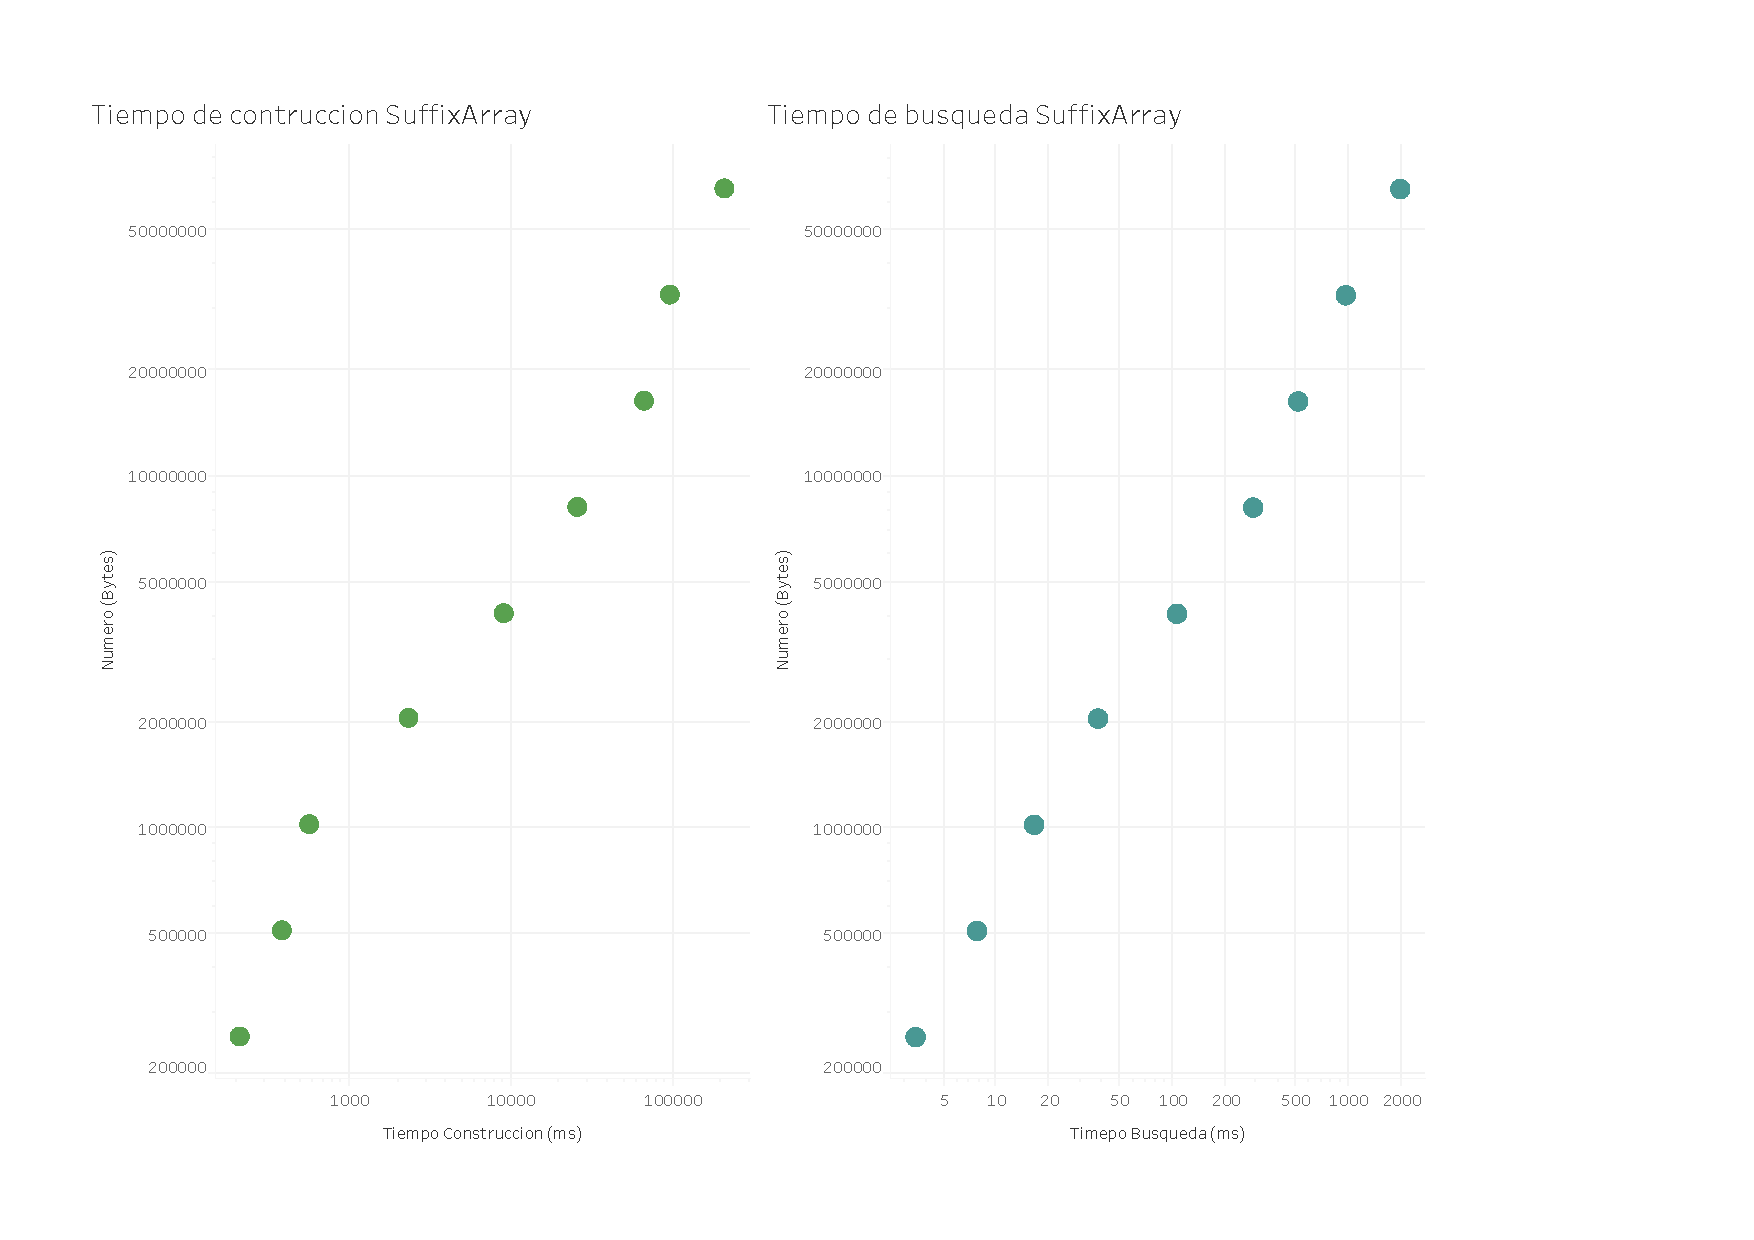
\includegraphics[width=0.8\textwidth]{figura1.pdf}

		Figura 1: Gráficos del tiempo de creación y búsqueda en el Suffix Array.
	\end{center}

	% % % % % % % % % % % % % % % % % % % % % % % % % % % % % % % % % % % % % % % % % % % % % % % % % % % % % % % % % % % % % % % % % % % % % % % % % % % % % % % % % % % % % % % % % %
	\newpage
	% % % % % % % % % % % % % % % % % % % % % % % % % % % % % % % % % % % % % % % % % % % % % % % % % % % % % % % % % % % % % % % % % % % % % % % % % % % % % % % % % % % % % % % % % %
\subsection{Tiempo de Creación y Búsqueda del Automata}

	Los resultados para los tiempos de construcción del Automata, fueron los siguientes.

	\begin{center}
		\begin{tabular}{|c|c|}
			\hline
			Tamaño del texto (Kb) ( & Tiempo de Construcción (ms)\\
			\hline
			$250$ & 0,014\\
			\hline
			$500$ & 0,011\\
			\hline
			$1000$ & 0,011\\
			\hline
			$2000$ & 0.012\\
			\hline
			$4000$ & 0.102\\
			\hline
			$8000$ & 0.029\\
			\hline
			$16000$ & 0.013\\
			\hline
			$32000$ & 0.031\\
			\hline
			$64000$ & 0.013\\
			\hline
			$128000$ & 0.092\\
			\hline
			$256000$ & 0.011\\
			\hline
		\end{tabular}
	\end{center}
	
	Para el caso de la búsqueda de una palabra el texto, los resultados fueron los siguientes.
	
	\begin{center}
		\begin{tabular}{|c|c|}
			\hline
			Tamaño del texto (Kb) ( & Tiempo de Búsqueda (ms)\\
			\hline
			$250$ & 3,199\\
			\hline
			$500$ & 5,909\\
			\hline
			$1000$ & 12,521\\
			\hline
			$2000$ & 25,595\\
			\hline
			$4000$ & 45,360\\
			\hline
			$8000$ & 117,171\\
			\hline
			$16000$ & 215,554\\
			\hline
			$32000$ & 776,584\\
			\hline
			$64000$ & 664,720\\
			\hline
			$128000$ & 1150,971\\
			\hline
			$256000$ & 2774,850\\
			\hline
		\end{tabular}
	\end{center}
	
	\newpage
    Se gráficaron estás dos tablas, los resultados son los siguientes.
	\begin{center}
		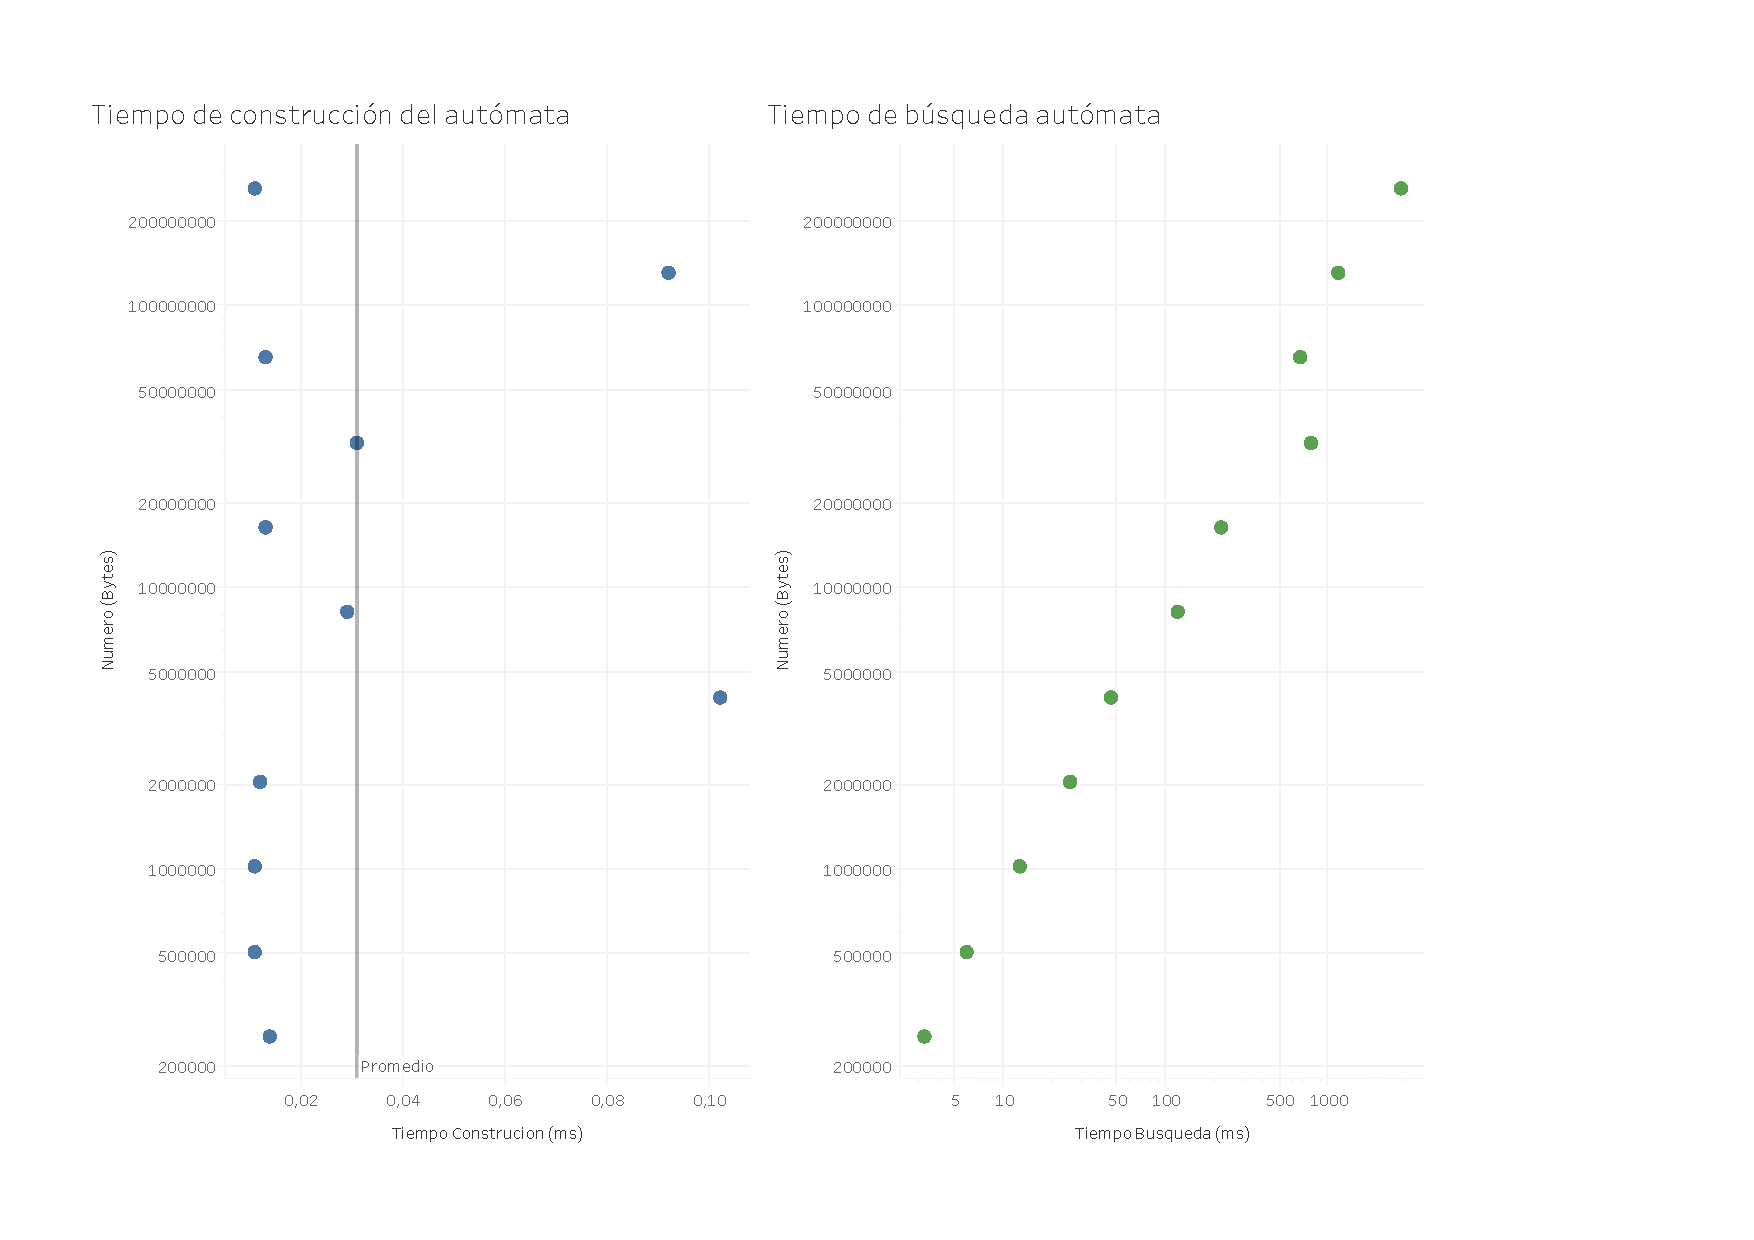
\includegraphics[width=0.8\textwidth]{figura2.pdf}

		Figura 2: Gráficos del tiempo de creación y búsqueda en el Automata.
	\end{center}
	% % % % % % % % % % % % % % % % % % % % % % % % % % % % % % % % % % % % % % % % % % % % % % % % % % % % % % % % % % % % % % % % % % % % % % % % % % % % % % % % % % % % % % % % % %
	\newpage
	% % % % % % % % % % % % % % % % % % % % % % % % % % % % % % % % % % % % % % % % % % % % % % % % % % % % % % % % % % % % % % % % % % % % % % % % % % % % % % % % % % % % % % % % % %

	\section{Análisis y Conclusiones}

	\subsection{Construcción del Suffix Array}
	
	Se observa del gráfico obtenido para la construcció que la implementación de la construcción del Suffix Array crece linealmente con el tamaño del texto, lo cual coincide con la hipótesis presentada al inicio del informe.


	\subsection{Búsqueda en el Suffix Array}
	
	Se observa del gráfico de la búsqueda del Suffix Array que el tiempo crece linealmente con el tamaño del texto, lo cual no coincide con la hipótesis que se habia presentado, revisando  el código se realizó la tranformación de cada sufijo a un arreglo de \textit{char} lo que toma $O(n)$, es por esto que se obtuvieron estos resultados.
    
    
    \subsection{Construcción del Automata}
	
	El grafico de la construcción del Automata no puede ser analisado debido a que no fueron registrados los largos del patrón, solo puede observarse que los tiempos de ejecución son muy pequeños.


	\subsection{Búsqueda en el Automata}
	
	Se observa del gráfico que la búsqueda de una palabra en el texto usando el algoritmo del Automata, que el tiempo crece linealmente con el tamaño del texto, lo cual coincide con la hipótesis que se habia presentado.



	\subsection{Conclusiones}
	
	La construcción del Suffix Array resultó igual al orden teórico que se conocia, para el caso del la búsqueda en él, se obtuvieron malos resultados debido a una mala implementación, debido a que en un paso del algoritmo se realizó un paso innecesario de la transformación de un \textit{String} a un arreglo de \textit{char} el cual hace que el timepo aumnete linealmente con la entrada, se corrigió este problema y se corrieron un número pequeños de experimentos (Anexo 1), en los cuales se podía observar la mejora del tiempo de búsqueda del algoritmo, pero al ser tan pocos experimentos no es concluyente.
	
	Para la construcción del Automata se realizaron de manera incorrecta los experimentos debido a que no se midió el largo del patron, se deberian haber repetido los experimentos, pero debido que el momento en que se detecto esta falla se estaba muy cerca de la fecha de entrega ya no quedaba tiempo para realizar un número suficiente de experimentos para obtener resultados convincentes. Aunque no se puede comparar el orden del algoritmo de construcción del Automata, si se puede observar que los tiempos de construcción en general fueron muy pequeños. La búsqueda en el Automata resultó del mismo orden del algoritmo teórico.\\
	
	Estas dos implementaciones funcionan para distintos propositos, el enfoque del Suffix Array tiene un orden lineal para construirse, pero posee un tiempo menor para la busqueda en el arreglo, por lo que debería ser usado en el caso de hacer muchas consultas sobre un texto. En el caso del Automata, la construcción toma muy poco tiempo pero correrlo sobre el texto es lineal al tamaño del texto, por lo que este enfoque puede ser usado cuando se quiere hacer pocas consultas sobre el texto.
	
	\newpage
	
	\section{Anexos}
        \subsection{Anexo 1}
        
		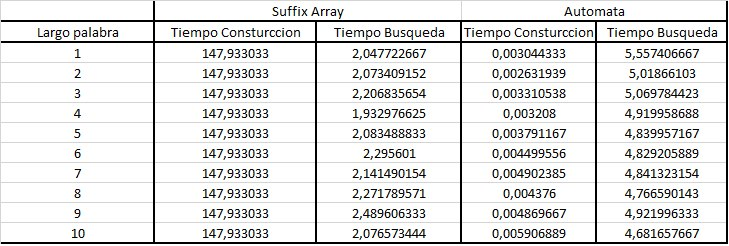
\includegraphics[width=0.8\textwidth]{figura3.jpg}

		Figura 3: Experimento con corrección de busqueda en Suffix Array texto de 1MB, con largo de palabra de 1 a 10.
       
	
	
	
	

\end{document}
